
\section{Simulation}
\label{sec:simulation}

We divided the simulation in 3 main parts (apart from the GUI): \\

\begin{itemize}
\item The driver model (chapter \ref{sec:driver})
\item The environment model (chapter \ref{sec:environment})
\item The vehicle model (chapter \ref{sec:vehicles})
\end{itemize} 

\noindent Figure \ref{fig:simulationProcess} shows how the different sections
of the simulation interact with each other.

\begin{figure}[H]
\begin{center}
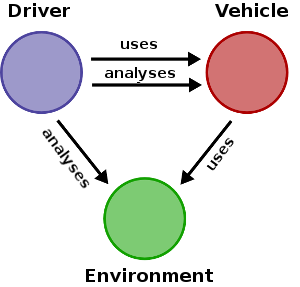
\includegraphics[scale=0.5]{images/process.png}
\end{center}
\caption{The interaction of the models}
\label{fig:simulationProcess}
\end{figure}

The core of the simulation is the event system, which is described in
the next chapter.

\subsection{The event system}
\label{sec:eventSystem}

The simulation is built as an event process, which means, that everything is
triggered through events that occur on a certain point in time.Currently,
there are following events implemented:

\begin{description}
\item[The driver event] This event can either indicate the driver
to assess his situation (\ref{sec:animus}) or contain a decision on the 
junction that his is approaching. The event that indicates an assessment
is created every few milliseconds, depending on the parameter in the driver's
physics (\ref{sec:physics}).
\item[The crash event]
This event indicates to the simulation that there has been a car crash.
\item[The vehicle event]
This event contains changes in the acceleration of the vehicle. With this 
event we simulate a delayed reaction of the driver.
\end{description}

\noindent All events are put into the event queue on creation. The queue sorts the
events according to their time stamps and are therefore processed in the
order that they have to occur. \\

\noindent Figure \ref{fig:eventSystem} shows the composition of the 
concerning classes. \\

\begin{figure}[H]
\begin{center}
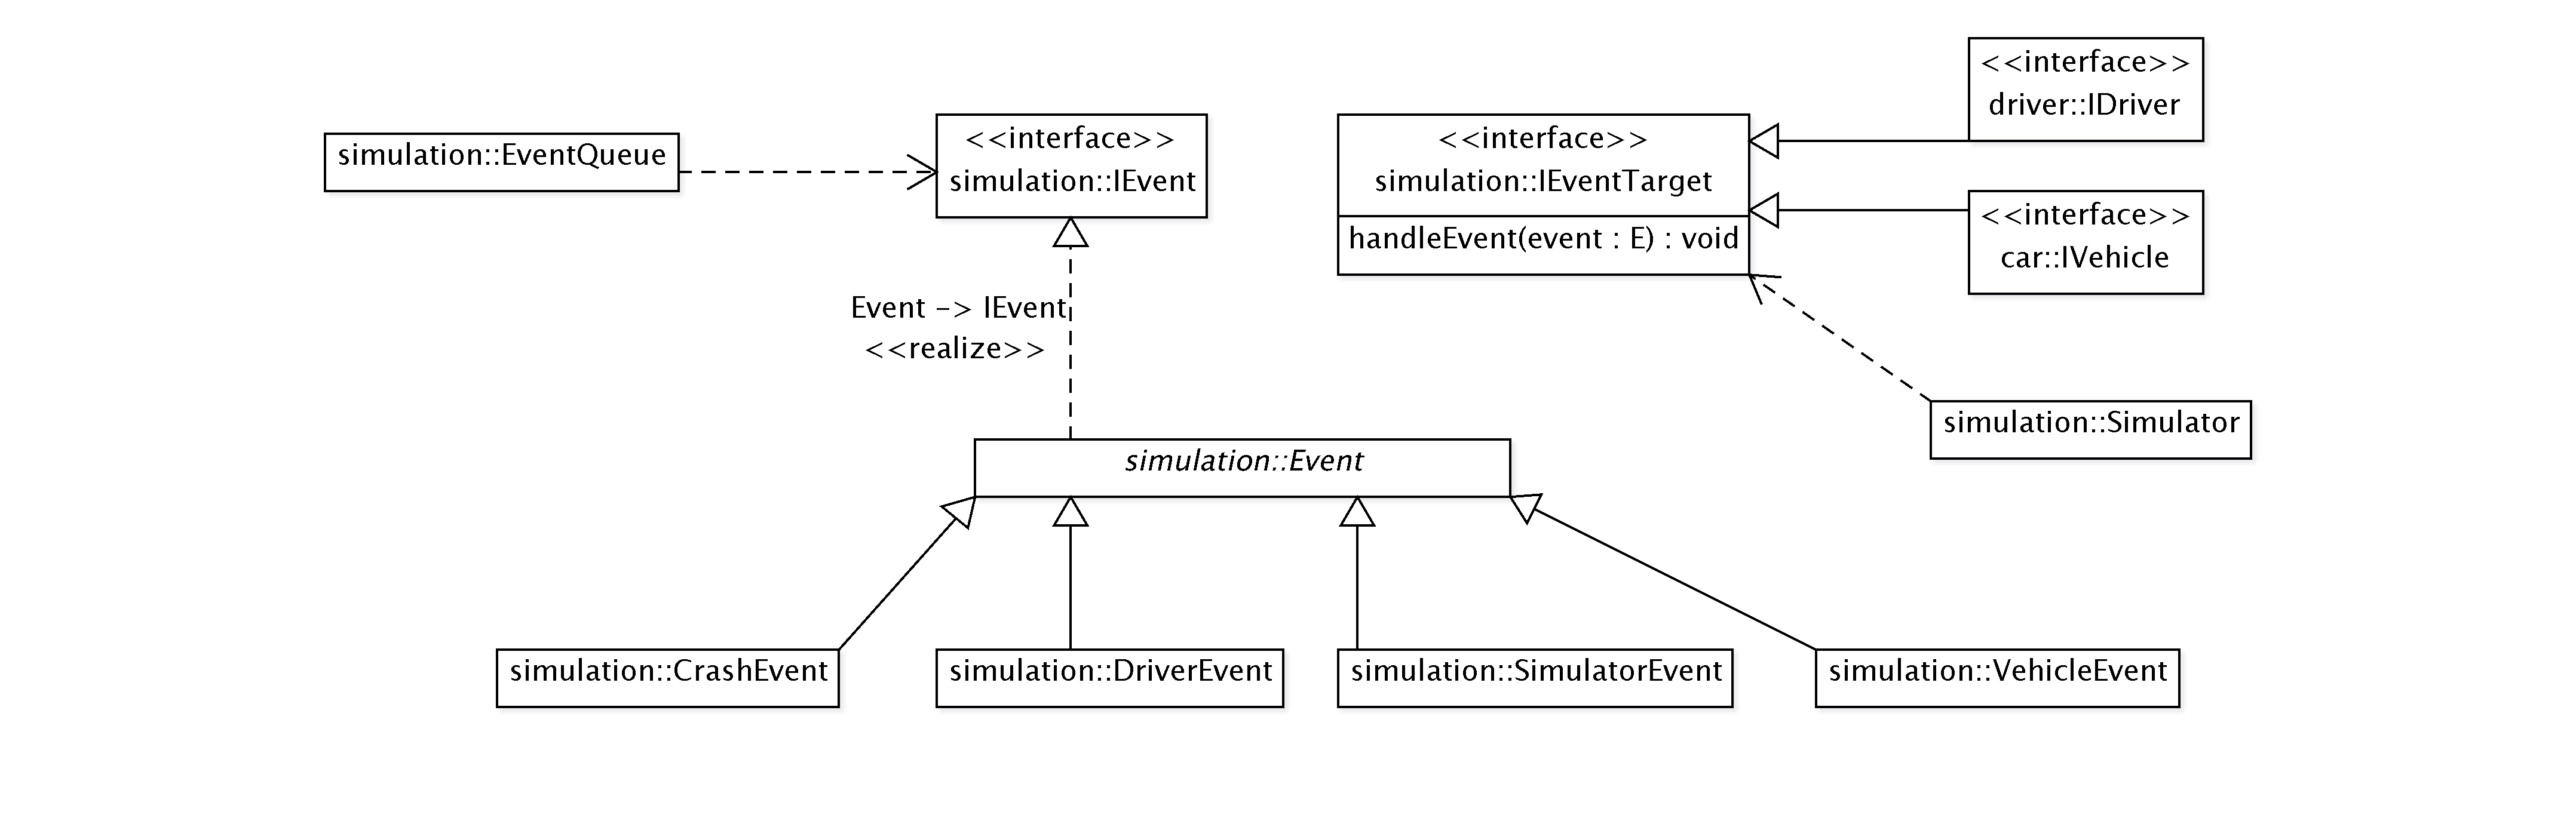
\includegraphics[width=\textwidth]{images/eventsystem.png}
\end{center}
\caption{The composition of the event system}
\label{fig:eventSystem}
\end{figure}

\subsection{The process}

The following figure shows how the main loop works:

\begin{figure}[H]
\begin{center}
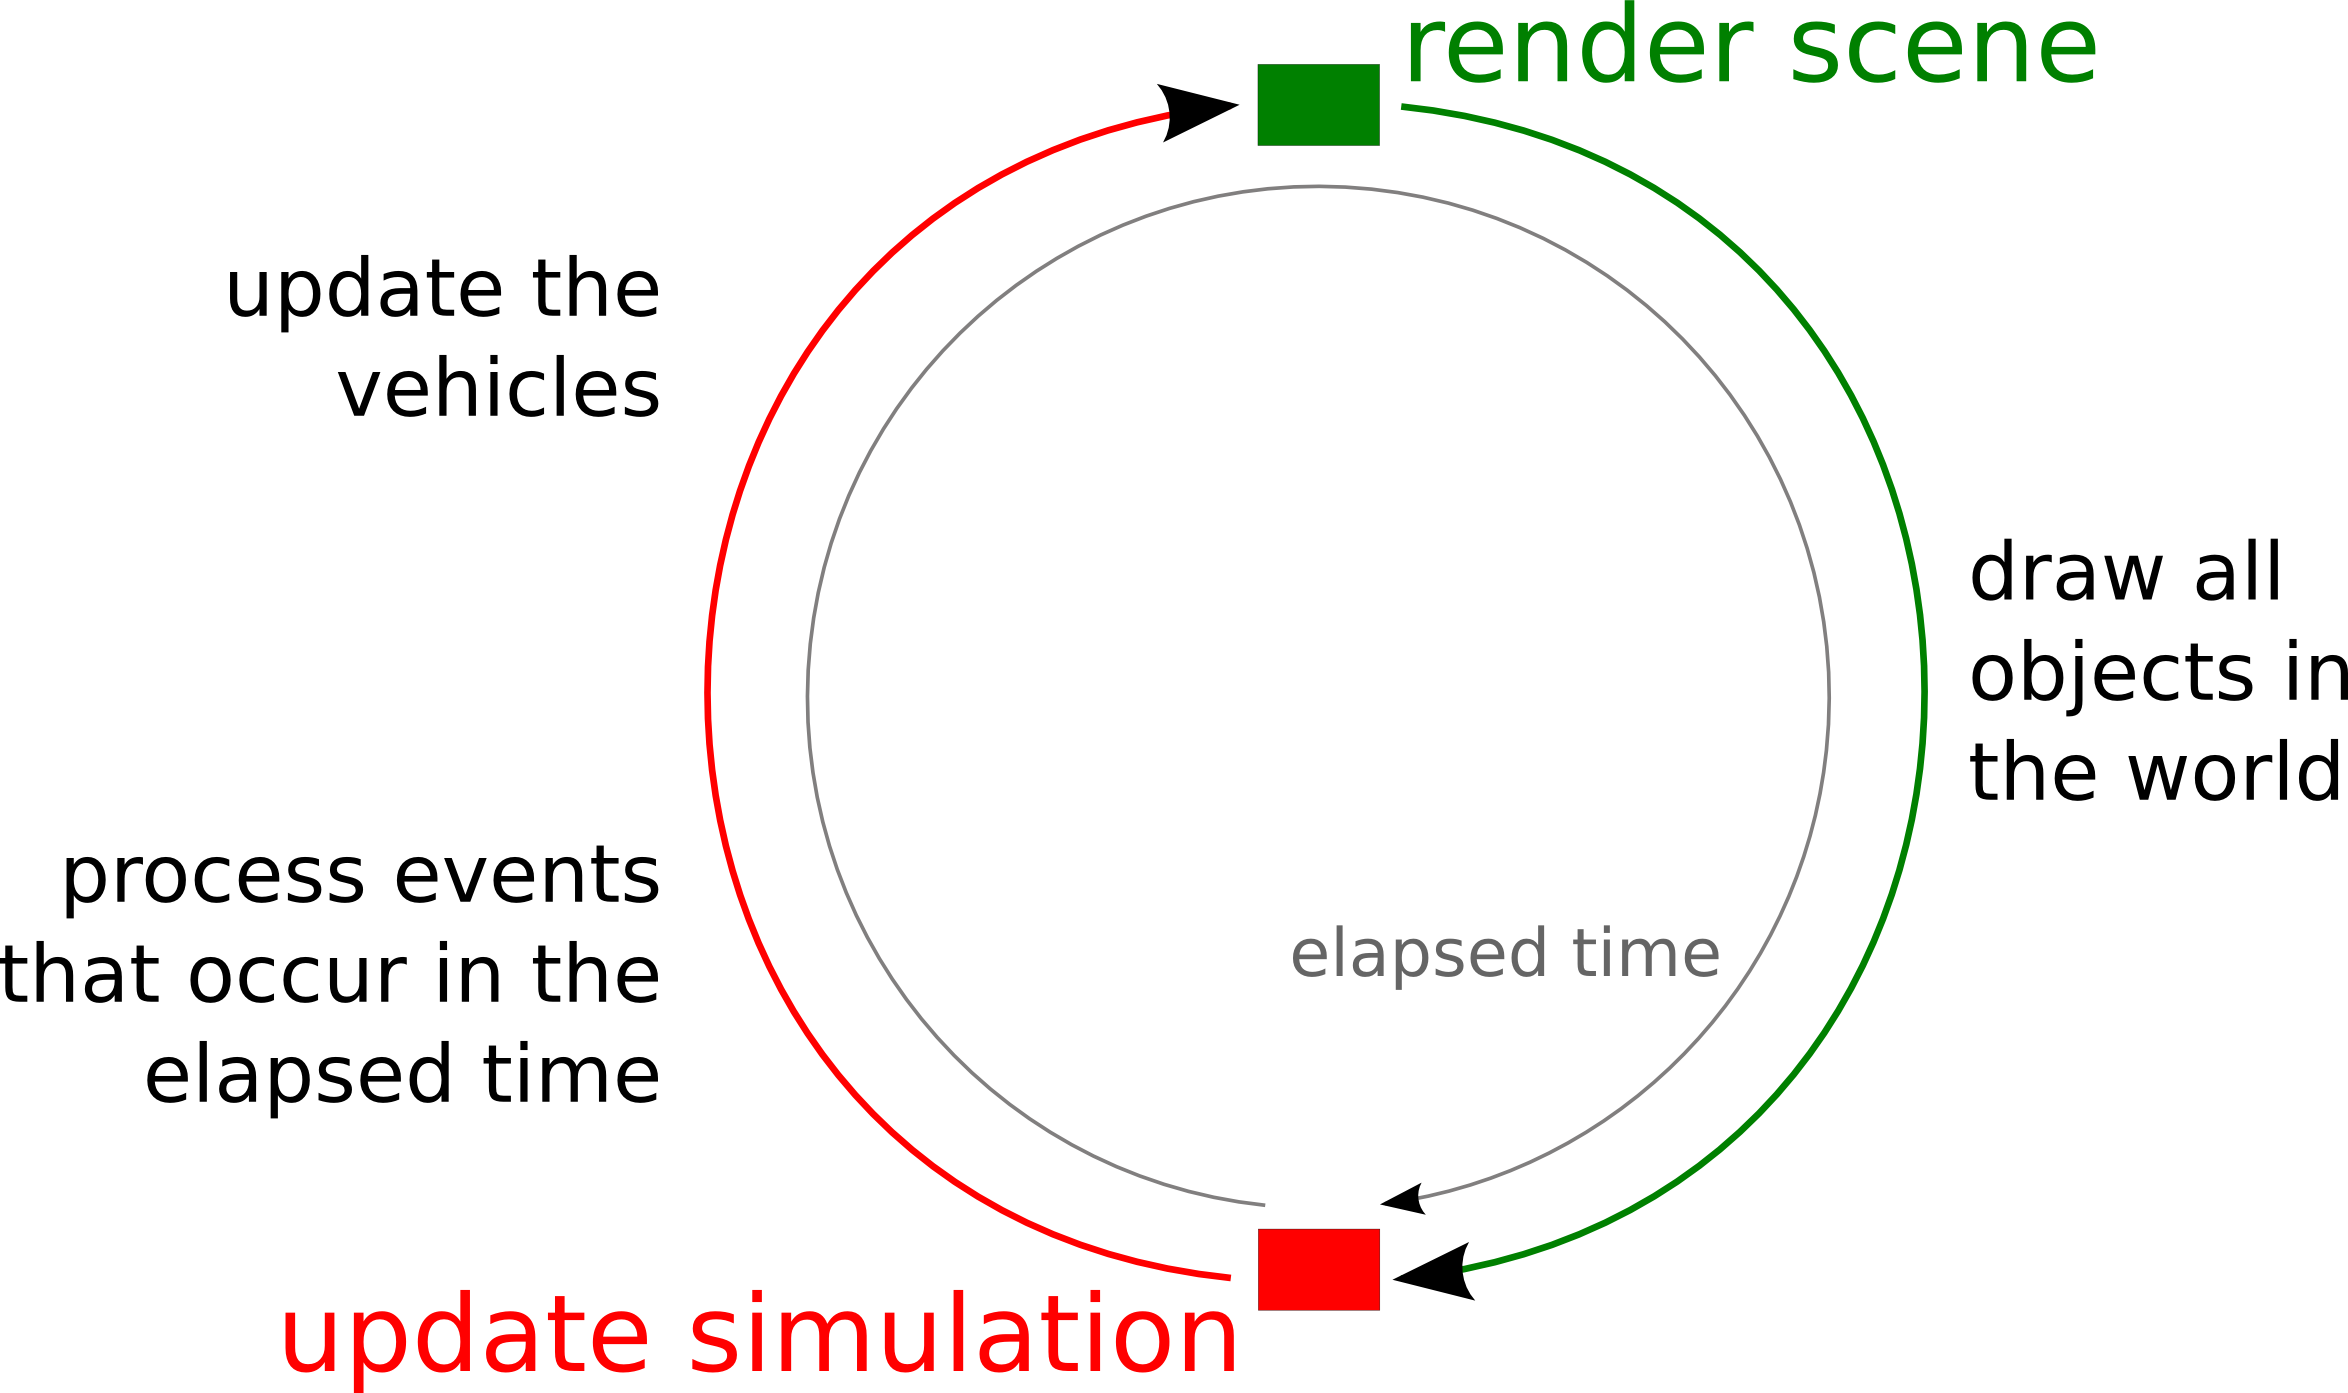
\includegraphics[scale=0.5]{images/simulationprocess.png}
\end{center}
\end{figure}

\noindent The simulation is heavily connected to the GUI (\ref{sec:gui}). Each
time a frame has been rendered, the GUI tells the simulation to update the 
world whereat it passes the elapsed time. The simulation then processes all
events that have to occur in that elapsed time, ordered by their time stamps.
With this model no threads are needed, and the GUI renders exactly the amount
% eer?
of frames possible to keep the simulation running.

